\documentclass[aspectratio=169, table]{beamer}

%\usepackage[beamertheme=./praditatheme]{Pradita}
\usepackage[utf8]{inputenc}
\usepackage{xcolor} % for color
\usepackage{colortbl} % for table color
\usepackage{listings}

% Define Java language style for listings
\lstdefinestyle{JavaStyle}{
language=Java,
basicstyle=\ttfamily\tiny,
keywordstyle=\color{blue},
commentstyle=\color{gray},
stringstyle=\color{red},
breaklines=true,
showstringspaces=false,
tabsize=2,
captionpos=b,
numbers=left,
numberstyle=\tiny\color{gray},
frame=lines,
backgroundcolor=\color{lightgray!10},
comment=[l]{//},
morecomment=[s]{/*}{*/},
commentstyle=\color{gray}\ttfamily,
string=[s]{'}{'},
morestring=[s]{"}{"},
%	stringstyle=\color{teal}\ttfamily,
%	showstringspaces=false
}

\lstdefinestyle{sql}{
language=sql,
keywords={use, insert, into, values, select, from,
update, set, delete, create, where, join, left, right, inner, order, by, primary, key},
ndkeywords={max, min, varchar, int},
ndkeywordstyle=\color{purple}\bfseries,
basicstyle=\ttfamily\scriptsize,
keywordstyle=\color{blue},
commentstyle=\color{gray},
stringstyle=\color{red},
breaklines=true,
showstringspaces=false,
tabsize=2,
captionpos=b,
numbers=left,
numberstyle=\tiny\color{gray},
frame=lines,
backgroundcolor=\color{lightgray!10},
comment=[l]{\#},
morecomment=[s]{/*}{*/},
commentstyle=\color{gray}\ttfamily,
string=[s]{'}{'},
morestring=[s]{"}{"},
%	stringstyle=\color{teal}\ttfamily,
%	showstringspaces=false
}

\lstdefinelanguage{bash} {
keywords={},
basicstyle=\ttfamily\scriptsize,
keywordstyle=\color{blue}\bfseries,
ndkeywords={iex},
ndkeywordstyle=\color{purple}\bfseries,
sensitive=true,
commentstyle=\color{gray},
stringstyle=\color{red},
numbers=left,
numberstyle=\tiny\color{gray},
breaklines=true,
frame=lines,
backgroundcolor=\color{lightgray!10},
tabsize=2,
comment=[l]{\#},
morecomment=[s]{/*}{*/},
commentstyle=\color{gray}\ttfamily,
stringstyle=\color{purple}\ttfamily,
showstringspaces=false
}

\lstdefinestyle{XmlStyle} {
language=xml,
keywords={xmlns,version,type,import},
basicstyle=\ttfamily\scriptsize,
keywordstyle=\color{blue}\bfseries,
ndkeywords={import},
ndkeywordstyle=\color{purple}\bfseries,
sensitive=true,
commentstyle=\color{gray},
stringstyle=\color{red},
numbers=left,
numberstyle=\tiny\color{gray},
breaklines=true,
frame=lines,
backgroundcolor=\color{lightgray!10},
tabsize=2,
showstringspaces=false,
comment=[l]{\#},
commentstyle=\color{gray}\ttfamily,
stringstyle=\color{purple}\ttfamily,
morecomment=[s]{<!--}{-->}
}

\lstdefinelanguage{css}{
basicstyle=\ttfamily\footnotesize,
keywordstyle=\color{blue},
commentstyle=\color{gray},
stringstyle=\color{red},
breaklines=true,
showstringspaces=false,
tabsize=2,
captionpos=b,
numbers=left,
numberstyle=\tiny\color{gray},
frame=lines,
backgroundcolor=\color{lightgray!10},
comment=[l]{//},
morecomment=[s]{/*}{*/},
commentstyle=\color{gray}\ttfamily,
string=[s]{'}{'},
morestring=[s]{"}{"},
%	stringstyle=\color{teal}\ttfamily,
%	showstringspaces=false
}

\lstdefinelanguage{puml}{
	basicstyle=\ttfamily\footnotesize,
	keywords={@startuml, @enduml, class, String, abstract, interface, Person, note, of, end, enum},
	ndkeywords={right, left},
	morekeywords={\{,\}, <!-- },
	emph={=,!,?}, emphstyle=\color{red}\bfseries,
	keywordstyle=\color{blue},
	commentstyle=\color{gray},
	stringstyle=\color{teal},
	ndkeywordstyle=\color{purple}\bfseries,
	breaklines=true,
	showstringspaces=false,
	tabsize=2,
	captionpos=b,
	numbers=left,
	numberstyle=\tiny\color{gray},
	frame=lines,
	backgroundcolor=\color{lightgray!10},
	comment=[l]{\'},
	morecomment=[s]{/*}{*/},
	commentstyle=\color{gray}\ttfamily,
	%	string=[s]{'}{'},
	morestring=[s]{"}{"},
	%	stringstyle=\color{teal}\ttfamily,
	%	showstringspaces=false
	literate=
	{\{}{{\textcolor{red}{\{}}}1
	{\}}{{\textcolor{red}{\}}}}1
	{:}{{\textcolor{red}{:}}}1
	{=}{{\textcolor{red}{=}}}1
}

\usetheme{Pradita}

\subtitle{IF220303 - Object-oriented Programming}

\title{\LARGE{Unified Modeling Language:}\\\LARGE{Structural Diagrams}\vspace{20pt}}
\date[Serial]{\scriptsize {PRU/SPMI/FR-BM-18/0222}}
\author[Pradita]{\small {\textbf{Alfa Yohannis}}}

\begin{document}

\frame{\titlepage}

\begin{frame}[fragile]
\frametitle{Contents}
\vspace{10pt}
\begin{columns}[t]
	\column{0.5\textwidth}
	\tableofcontents[sections={1-5}]
	
	\column{0.5\textwidth}
	\tableofcontents[sections={6-10}]
\end{columns}
\end{frame}

\section{Unified Modeling Language (UML)}

\begin{frame}{Unified Modeling Language (UML)}
	\vspace{20pt}
	Unified Modeling Language (UML) is a visual modeling standard used in software engineering to:
	\begin{itemize}
		\item \textbf{Describe} software systems visually.
		\item \textbf{Design} system architecture and components before implementation.
		\item \textbf{Document} system structure and behavior for maintenance and further development.
		\item \textbf{Help developers} understand the relationships between system components.
	\end{itemize}
\end{frame}

\section{History of UML}

\begin{frame}{History of UML}
	\vspace{20pt}
	UML was developed in the 1990s by integrating several existing software modeling methods, such as:
	\begin{itemize}
		\item \textbf{Booch Method} – Used for object-oriented system analysis and design.
		\item \textbf{OMT (Object Modeling Technique)} – Focused on object-based system modeling.
		\item \textbf{OOSE (Object-Oriented Software Engineering)} – Introduced the concept of \textit{use cases}.
	\end{itemize}
	In 1994, the \textbf{Three Amigos} (Grady Booch, James Rumbaugh, and Ivar Jacobson) developed UML as a unified modeling standard, which was later submitted to the OMG in 1997 for standardization.
\end{frame}

\section{Development and Applications of UML}

\begin{frame}{Development of UML}
	\vspace{20pt}
	After being approved by the OMG, UML continued to evolve with various revisions and improvements. Key milestones in its development include:
	\begin{itemize}
		\item \textbf{UML 1.0 (1997)} – The first version standardized by OMG.
		\item \textbf{UML 1.3 (1999)} – Enhancements in diagram elements and better support for object-based systems.
		\item \textbf{UML 2.0 (2005)} – Major improvements, including more diagram types and enhanced system behavior expression.
		\item \textbf{Latest UML versions} – Continuously updated by OMG to support advancements in software technology.
	\end{itemize}
\end{frame}

\begin{frame}{Applications of UML in Software Engineering}
	\vspace{20pt}
	Today, UML is widely used in various fields of software engineering, such as:
	\begin{itemize}
		\item Object-oriented system development.
		\item Modeling software architecture, designing databases, and distributed systems.
		\item A communication tool, particularly in software analysis, design, development, and deployment.
		\item Formal documentation of software projects.
	\end{itemize}
\end{frame}

\section{Software Modeling Tools}

\begin{frame}{Software Modeling Tools}
	\vspace{20pt}
	Software modeling enables developers to document, design, and understand a system before implementation. Various tools are used to create UML diagrams, including:
	\begin{itemize}
		\item \textbf{Enterprise Architect} – A professional tool for UML-based software architecture documentation and analysis.
		\item \textbf{StarUML} – An open-source tool with an interactive graphical interface for UML modeling.
		\item \textbf{Visual Paradigm} – Supports multiple UML diagrams with strong analysis and documentation features.
		\item \textbf{Draw.io} – A web-based tool for creating various diagrams, including UML.
		\item \textbf{PlantUML} – A text-based modeling tool for creating UML diagrams using simple scripts.
	\end{itemize}
\end{frame}

\begin{frame}{PlantUML: A Text-Based Modeling Tool}
	\vspace{20pt}
	\textbf{PlantUML} allows users to create UML diagrams using a text-based syntax. Unlike graphical interface-based tools, PlantUML follows a declarative approach where text-based code is rendered into visual diagrams.
	
	\textbf{Advantages of PlantUML:}
	\begin{itemize}
		\item \textbf{Text-Based} – Easily integrated with version control systems such as Git.
		\item \textbf{Supports Various UML Diagrams} – Including \textit{class diagrams}, \textit{sequence diagrams}, \textit{component diagrams}, and more.
		\item \textbf{Wide Integration} – Can be used in editors like VS Code, IntelliJ IDEA, Eclipse, and integrated into LaTeX or Markdown documents.
		\item \textbf{Lightweight and Easy to Use} – Does not require a graphical interface, only simple text scripts.
	\end{itemize}
\end{frame}


\begin{frame}{Class Diagram}
	\vspace{20pt}
	\centering
	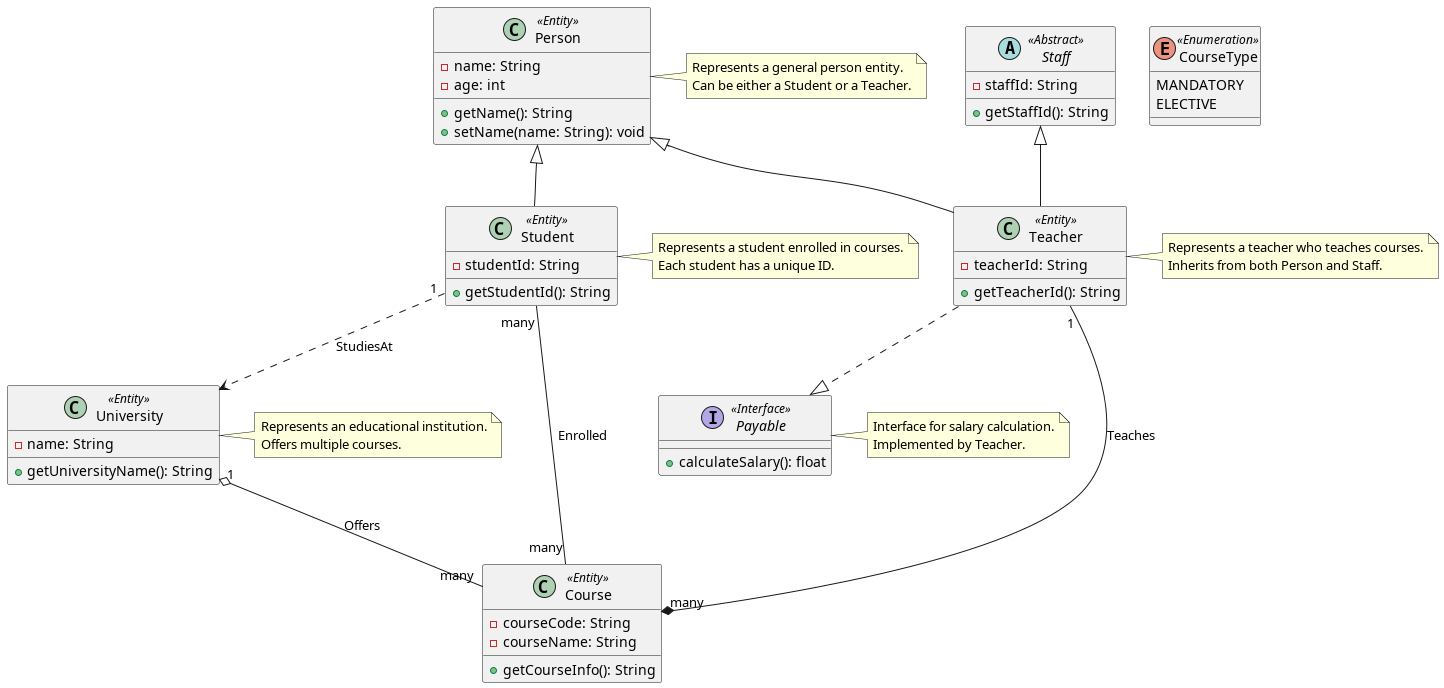
\includegraphics[width=\textwidth]{../../figures/out/class_diagram.png}
\end{frame}

\begin{frame}{Object Diagram}
	\vspace{20pt}
	\centering
	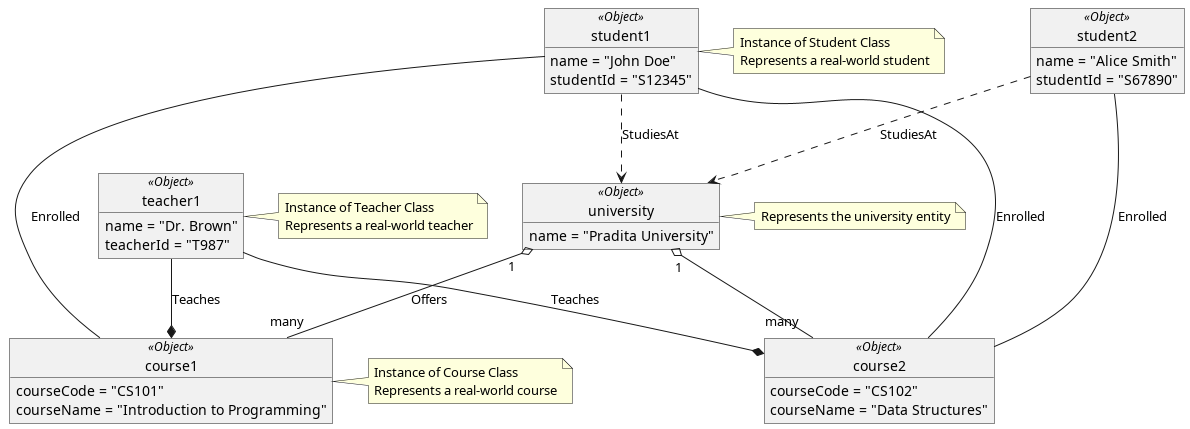
\includegraphics[width=\textwidth]{../../figures/out/object_diagram.png}
\end{frame}

\begin{frame}{Component}
	\framesubtitle{Diagram}
	\centering
	\vspace{-5pt}
	\hspace{10pt}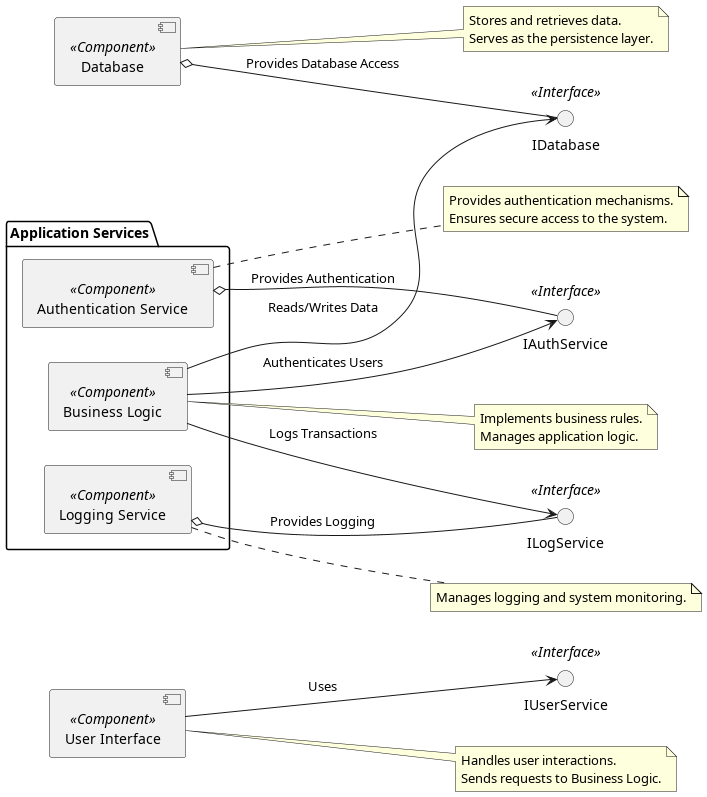
\includegraphics[width=.55\textwidth]{../../figures/out/component_diagram.png}
\end{frame}

\begin{frame}{Deployment Diagram}
	\vspace{30pt}
	\centering
	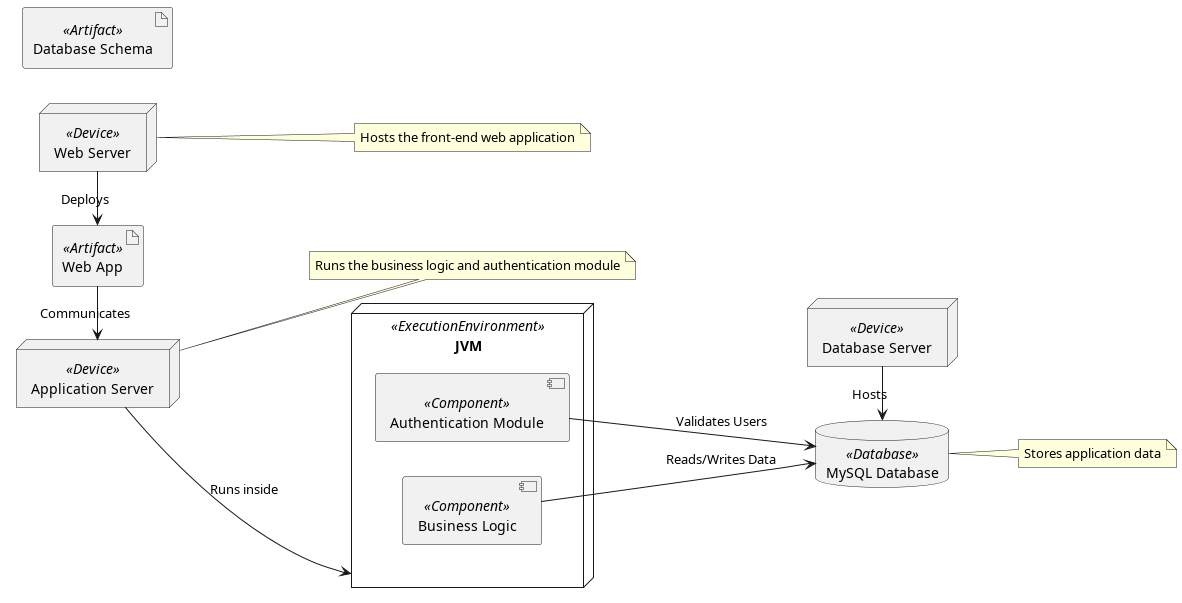
\includegraphics[width=\textwidth]{../../figures/out/deployment_diagram.png}
\end{frame}

\section{References}

\begin{frame}{References}
	\vspace{20pt}
	For a more in-depth study of UML, please visit the following link:  
	\url{https://www.uml-diagrams.org/}
\end{frame}


\end{document}
